\hypertarget{main_8cpp}{
\section{Dokumentacja pliku /home/pawel/Dokumenty/Uczelnia/grupappz/Source/Ass8-server/main.cpp}
\label{main_8cpp}\index{/home/pawel/Dokumenty/Uczelnia/grupappz/Source/Ass8-server/main.cpp@{/home/pawel/Dokumenty/Uczelnia/grupappz/Source/Ass8-server/main.cpp}}
}
{\tt \#include $<$iostream$>$}\par
{\tt \#include $<$string$>$}\par
{\tt \#include $<$cstdio$>$}\par
{\tt \#include $<$cstdlib$>$}\par
{\tt \#include $<$sys/types.h$>$}\par
{\tt \#include $<$unistd.h$>$}\par
{\tt \#include $<$sys/wait.h$>$}\par
{\tt \#include $<$boost/asio.hpp$>$}\par
{\tt \#include $<$boost/thread/thread.hpp$>$}\par
{\tt \#include $<$boost/bind.hpp$>$}\par
{\tt \#include \char`\"{}version.h\char`\"{}}\par
{\tt \#include \char`\"{}parser.hpp\char`\"{}}\par


Wykres zależności załączania dla main.cpp:\nopagebreak
\begin{figure}[H]
\begin{center}
\leavevmode
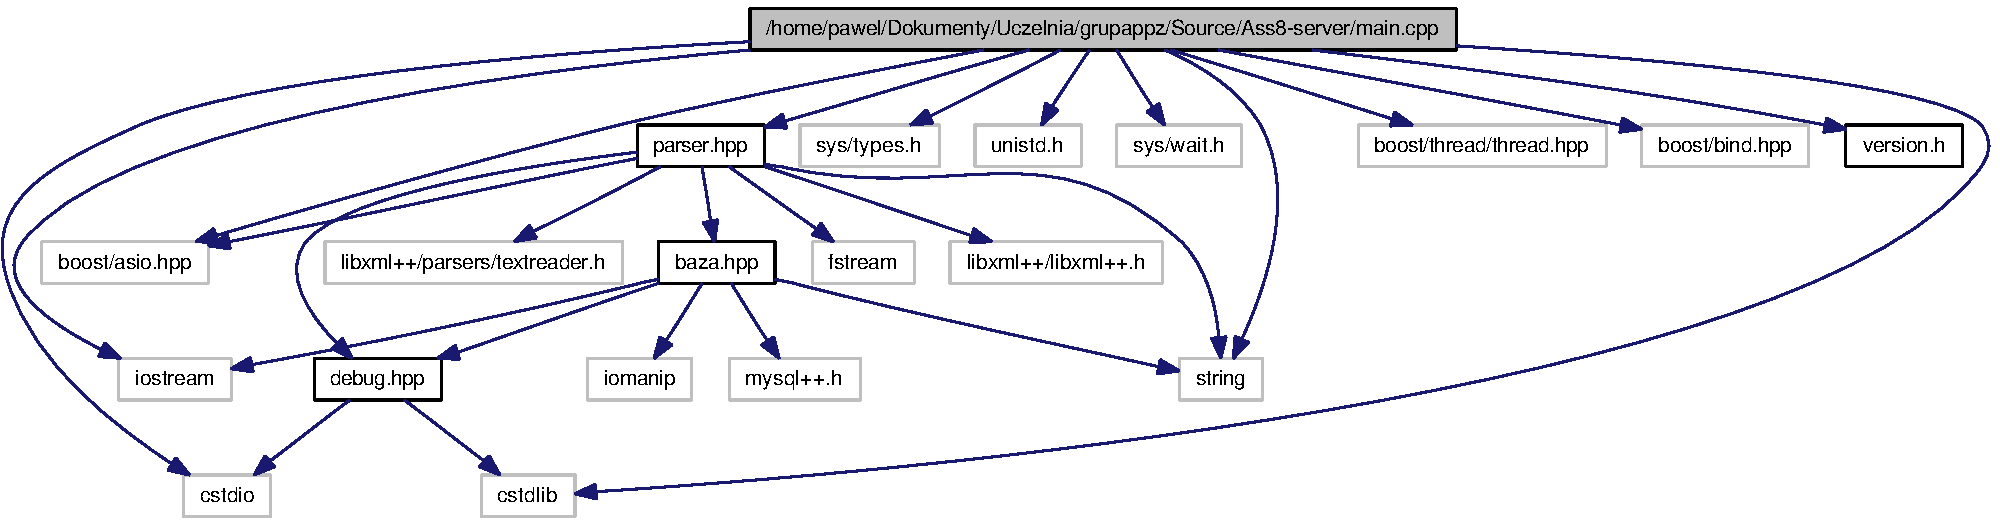
\includegraphics[width=420pt]{main_8cpp__incl}
\end{center}
\end{figure}
\subsection*{Funkcje}
\begin{CompactItemize}
\item 
int \hyperlink{main_8cpp_0ddf1224851353fc92bfbff6f499fa97}{main} (int argc, char $\ast$argv\mbox{[}$\,$\mbox{]})
\end{CompactItemize}


\subsection{Dokumentacja funkcji}
\hypertarget{main_8cpp_0ddf1224851353fc92bfbff6f499fa97}{
\index{main.cpp@{main.cpp}!main@{main}}
\index{main@{main}!main.cpp@{main.cpp}}
\subsubsection[{main}]{\setlength{\rightskip}{0pt plus 5cm}int main (int {\em argc}, \/  char $\ast$ {\em argv}\mbox{[}$\,$\mbox{]})}}
\label{main_8cpp_0ddf1224851353fc92bfbff6f499fa97}




Zmienna przechowująca port na którym serwer nasłucuje

Zmienne przechowujące parametry podłączenia do bazy danych

Zmienna przechowująca nazwę bazy w bazie danych

Jeżeli jest mniej niż 5 argumentów

To kończymy program

Potrzebne do połączenia z klientem

Potrzebne do połączenia z klientem

Potrzebne do połączenia z klientem

Watek ktory bedzie usuwal skonczone forki

Nieskonczona pętla

Wyjście/Wejście socketa

utworzenie parsera w forku (dla każdego klienta jeden taki jest tworzony); 

Definicja w linii 30 pliku main.cpp.

Oto graf wywołań dla tej funkcji:\nopagebreak
\begin{figure}[H]
\begin{center}
\leavevmode
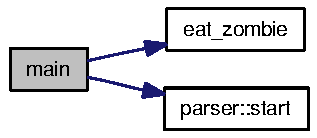
\includegraphics[width=94pt]{main_8cpp_0ddf1224851353fc92bfbff6f499fa97_cgraph}
\end{center}
\end{figure}
